\subsubsection{Process Hierarchy}
\emph{Google Chrome} uses a special process hierarchy to reduce the risk of an attack onto the browser. \emph{Chrome} creates multiple processes to isolate different contexts. A context can represent a (web-)site, a site instance or a tab \cite{chromium_process_models}. Depending on the chosen command line flag, the respective context is chosen and processes are created. To share data between the processes, inter process communication is used.
\begin{figure}[h]
\centering
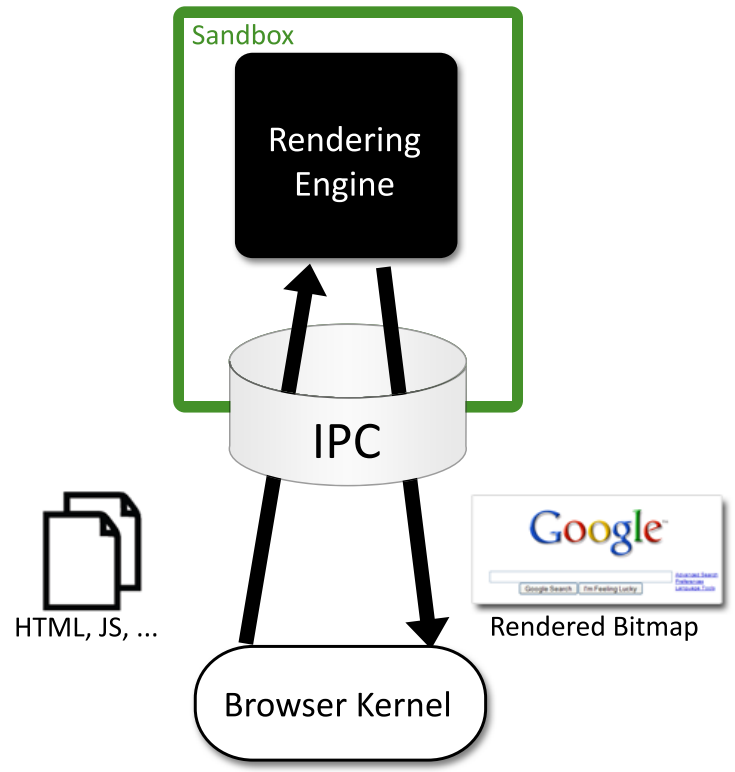
\includegraphics[scale=0.5]{sections/background/chrome/communication.png}
\caption{Communication between \emph{Browser Kernel} and the \emph{Rendering Engine}. The \emph{Rendering Engine} is used as a blackbox \cite{chromium_security_architecture}}
\label{fig:chrome_communication}
\end{figure}
Figure~\ref{fig:chrome_communication} shows the communication between \emph{Chrome's} processes. The \emph{Rendering Engine} is considered a blackbox which gets sent the received server response. A bitmap is generated and sent back to the \emph{Browser Kernel} process, from where the bitmap can be displayed to the user. Primarily a named pipe \cite{chromium_security_architecture} is used for this inter process communication. However, \emph{Chrome's} source code shows usages of the \syscall{WriteProcessMemory} function, which is used for inter process communication as well. \syscall{WriteProcessMemory} is hereby used to patch function calls. \cite{chromium_source_writeprocessmemory} shows 16 occurrences of the \syscall{WriteProcessMemory} function in \emph{Chrome's} source code.